\documentclass[a4paper]{article}

%% Language and font encodings
\usepackage[english]{babel}
\usepackage[utf8x]{inputenc}
\usepackage[T1]{fontenc}
\usepackage{caption}
\usepackage{subcaption}
\usepackage{color,soul}

%% Sets page size and margins
\usepackage[a4paper,top=3cm,bottom=2cm,left=3cm,right=3cm,marginparwidth=1.75cm]{geometry}

%% Useful packages
\usepackage{amsmath}
\usepackage{graphicx}
\usepackage{adjustbox}
\usepackage[colorinlistoftodos]{todonotes}
\usepackage[colorlinks=true, allcolors=blue]{hyperref}
\usepackage{float} % here for H placement parameter
\usepackage{hyperref}
\usepackage{verbatim}
\usepackage{varwidth}

\title{Analysis of the stochastic spread of Stride
simulation  outcomes.}
\author{Episim}
\date{April 22, 2018}

\begin{document}
\maketitle

\begin{abstract}
\noindent
The goal of this paper is to determine the stochastic spread of Stride simulation outcomes and find boundaries for testing purposes. We will discuss the following use cases (diseases).\\
\begin{itemize}
\item Influenza A
\item Influenza C
\item Measles (R0 is 12)
\item Measles (R0 is 16)
\\
\end{itemize}
\end{abstract}
\section{Configuration and data files}
These files are used in all our test runs. \\
The files are found in our repo and under the provided link.
\\
\begin{itemize}
\item  \href{https://github.com/RobbeHeirman/Configs/blob/master/config/geogen_default.xml}{GeoGen config} Config of geogen.
\item \href{https://github.com/RobbeHeirman/Configs/blob/master/data/flanders_cities.csv}{Flanders Cities} data for relative pop of flanders.
\item \href{https://github.com/RobbeHeirman/Configs/blob/master/data/flanders_commuting.csv}{Flanders Commuting} commuting info of flander cities.
\item \href{https://github.com/RobbeHeirman/Configs/blob/master/data/households_flanders.xml}{Household Flanders} household sample data.
\end{itemize}
\section{Scripts}
We used 3 extra scripts to gather data and compile the gathered data into images and results.

\subsection{SeedGenerator.py}
Found \href{https://github.com/RobbeHeirman/Configs/blob/master/Scripts/seedGenerator.py}{here}.
Helper script to generate a given amount of random seeds. Written to a .txt file. Same format as Seedtester will use to generate data off seeds.

\subsection{SeedTester.py}
Found \href{https://github.com/RobbeHeirman/Configs/blob/master/Scripts/seedTester.py}{here}.\\
This script will run stride with the config files and seed.txt file provided. Running stride for n given days. It will output for each seed the seed and amount of infected to a .dat files (referenced later).

\subsection{Plotter.py}
Found \href{https://github.com/RobbeHeirman/Configs/blob/master/Scripts/plotter.py}{here}.
This will generate for each .dat file in seedTesterResults a:
\begin{itemize}
\item box plot
\item histogram
\item QQ-plot
\item Scatter plot
\item A data file containing useful data like variance, mean and boundaries...
\end{itemize}

\section{Quantifying boundaries}
In our previous paper we already concluded that the number of threads and choice of random number generators did not have a large impact on end results. In this paper we will not attempt to analyze all data with every different thread/generator configuration. Instead we used lcg64 and 1 thread (sequential) in all our test cases.
\\
\\
In this section we will discuss the results of each of the above given use cases and try to decide boundaries of our data. Notable parameters are. The population is of size 600 000 and we used 30 steps (simulated days) for each run.

\noindent Plotter.py compiles some useful information about the runs on Influenza A. First off we inspect our QQ plot. The data tends to follow the line so we could assume if our sample set is bigger the data converges to a normal distribution for all use cases.
\\
\\
A naive interpretation  to set boundaries  is to take the lower and upper bound each sample. This is insufficient since we only tested a small sample size and it is still possible there are outliers.
\\
\\
Another approach we attempted is to make use of a BTI to take as data points. So we could assume 99\% of the cases would fall with in the BTI. But in practice, in some cases the tests still gave False negatives.
\\
\\
The last approach, is to calculate a "margin" parameter (that is also used in \href{https://github.com/RobbeHeirman/Episim/blob/master/test/cpp/gtester/BatchRuns.cpp}{BatchRuns.cpp} for use cases).
Margin represents a fraction of how much a result can be off the average or "expected result".
This method seemed to be fool proof on False negatives. And it is reasonable to say that the given margin is not to big for False positives.\\\\
Formula to calculate the margin:\\

\[ml = (mean -lower_bound) / mean\]
\[mh = (higher_bound - mean) / mean \]
\[margin = max(ml,mh)\]
\\
\\
What follows are the results our plotter script compiled for each of the use cases. What's most important is to take a look at the distribution and the calculated "Batchruns.cpp" margin value.
\pagebreak

\subsection{Influenza A}
Stride config file found \href{https://github.com/RobbeHeirman/Configs/blob/master/config/run_random-geopop_nolog-influAtest.xml}{here}.\\
Use of this \href{https://github.com/RobbeHeirman/Configs/blob/master/100-random.txt}{seed file}.
\\
\verbatiminput{Influenza_A/Influenza_A-data.txt}
\begin{figure}[H]
\centering
\begin{subfigure}{.5\textwidth}
  \centering
  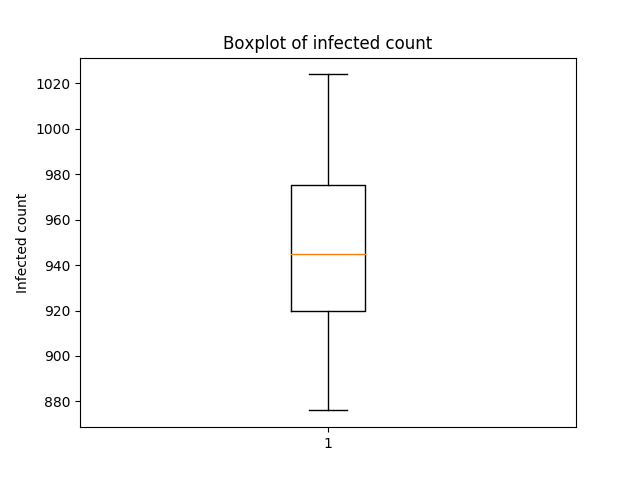
\includegraphics[width=1\linewidth]{Influenza_A/Influenza_A-boxplot.png}
  \caption{Boxplot of the Influenza A runs}
  \label{fig:Boxplot_Influenza_A}
\end{subfigure}%
\begin{subfigure}{.5\textwidth}
  \centering
  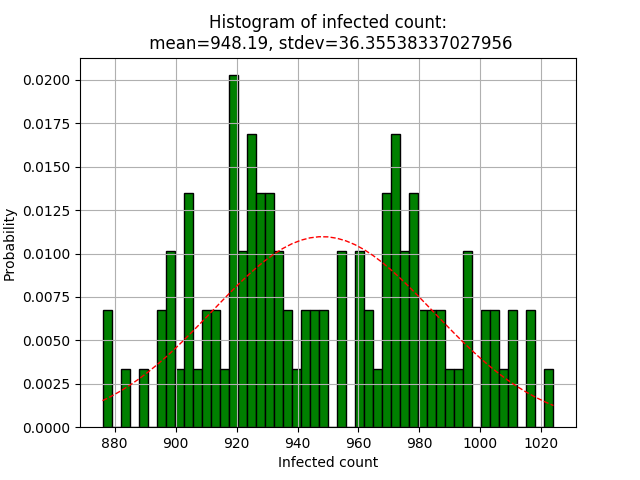
\includegraphics[width=1\linewidth]{Influenza_A/Influenza_A-histogram.png}
  \caption{Histogram of the Influenza A runs}
  \label{fig:Histogram_Influenza_A}
\end{subfigure}

\begin{subfigure}{.5\textwidth}
  \centering
  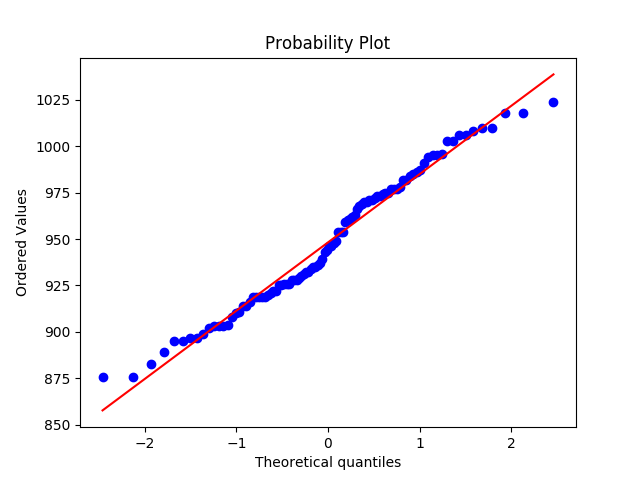
\includegraphics[width=1\linewidth]{Influenza_A/Influenza_A-qqplot.png}
  \caption{QQ-plot of Influenza A}
  \label{fig:QQ-plot_Influenza_A}
\end{subfigure}%
\begin{subfigure}{.5\textwidth}
  \centering
  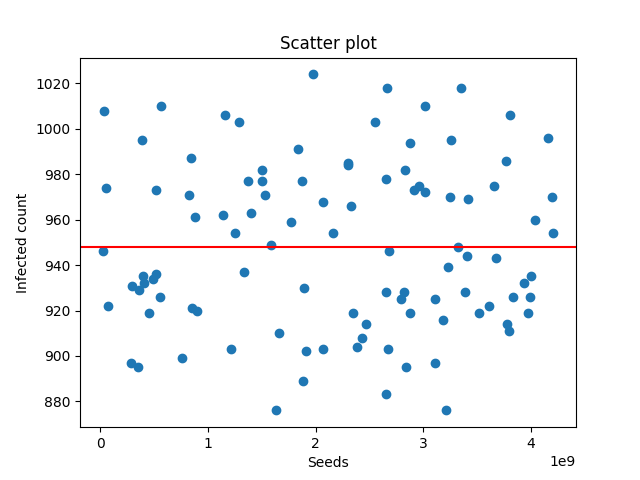
\includegraphics[width=1\linewidth]{Influenza_A/Influenza_A-scatterplot.png}
  \caption{Scatter plot of Influenza A}
  \label{fig:scatterplot_Influenza_A}
\end{subfigure}
\caption{Figures of Influenza A}
\label{fig:Influenza_A }
\end{figure}
\pagebreak
%-------------------------------

\subsection{Influenza C}
Stride config file found \href{https://github.com/RobbeHeirman/Configs/blob/master/config/run_random-geopop_nolog-influC.xml}{here}.\\
Use of this \href{https://github.com/RobbeHeirman/Configs/blob/master/100-random.txt}{seed file}.
\\
\verbatiminput{Influenza_C/Influenza_C-data.txt}
\begin{figure}[H]
\centering
\begin{subfigure}{.5\textwidth}
  \centering
  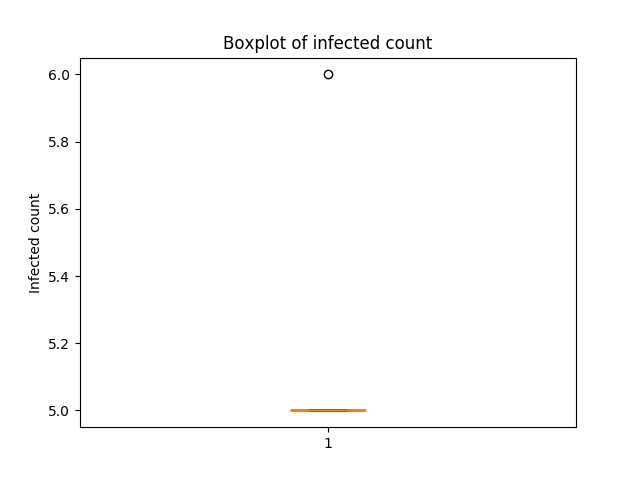
\includegraphics[width=1\linewidth]{Influenza_C/Influenza_C-boxplot.png}
  \caption{Boxplot of the Influenza C runs}
  \label{fig:Boxplot_Influenza_C}
\end{subfigure}%
\begin{subfigure}{.5\textwidth}
  \centering
  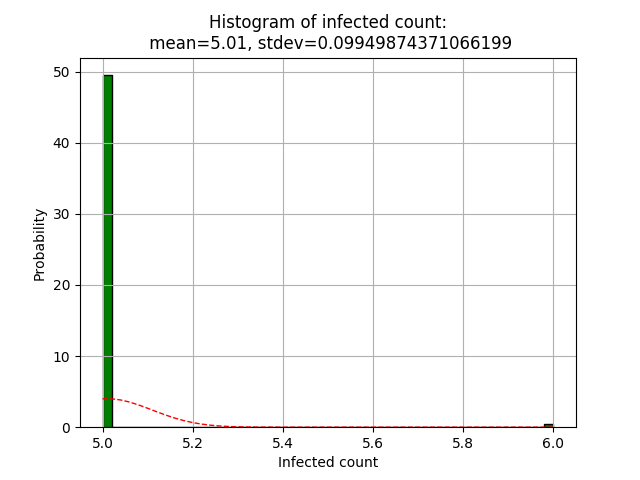
\includegraphics[width=1\linewidth]{Influenza_C/Influenza_C-histogram.png}
  \caption{Histogram of the Influenza C runs}
  \label{fig:Histogram_Influenza_C}
\end{subfigure}

\begin{subfigure}{.5\textwidth}
  \centering
  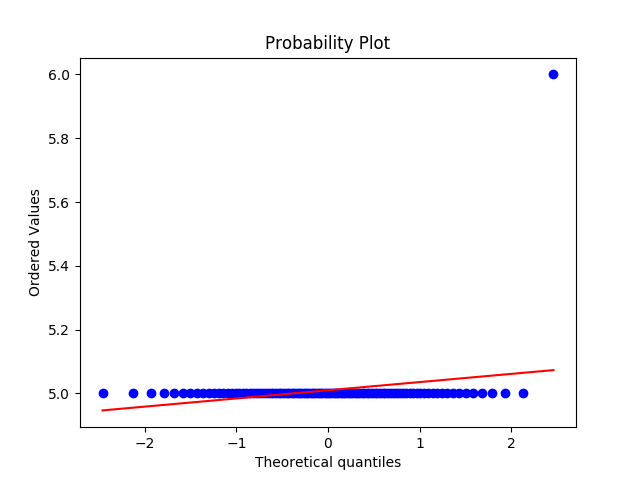
\includegraphics[width=1\linewidth]{Influenza_C/Influenza_C-qqplot.png}
  \caption{QQ-plot of Influenza C}
  \label{fig:QQ-plot_Influenza_C}
\end{subfigure}%
\begin{subfigure}{.5\textwidth}
  \centering
  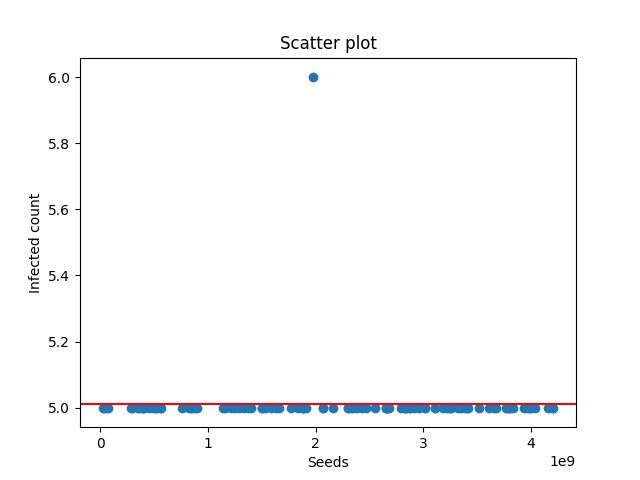
\includegraphics[width=1\linewidth]{Influenza_C/Influenza_C-scatterplot.png}
  \caption{Scatter plot of Influenza C}
  \label{fig:scatterplot_Influenza_C}
\end{subfigure}
\caption{Figures of Influenza C}
\label{fig:Influenza_C }
\end{figure}
\pagebreak
%-----------------
\subsection{Measles 12}
Stride config file found \href{https://github.com/RobbeHeirman/Config1s/blob/master/config/run_random-geopop_nolog-measles.xml}{here}.\\
Use of this \href{https://github.com/RobbeHeirman/Configs/blob/master/100-random.txt}{seed file}.
\\
\verbatiminput{Measles_12/Measles_12-data.txt}
\begin{figure}[H]
\centering
\begin{subfigure}{.5\textwidth}
  \centering
  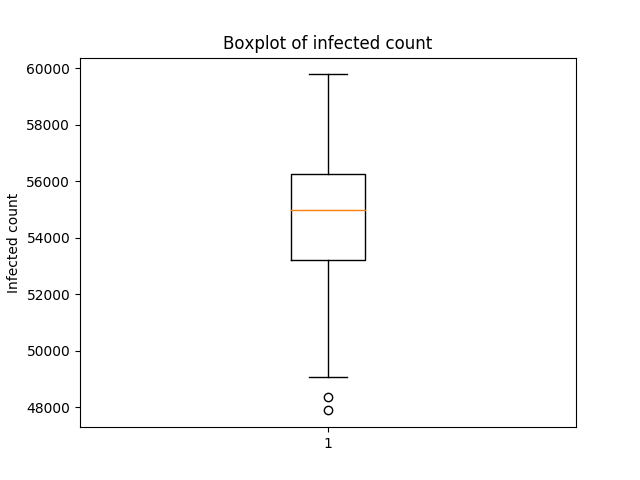
\includegraphics[width=1\linewidth]{Measles_12/Measles_12-boxplot.png}
  \caption{Boxplot Measles 12 runs }
  \label{fig:Boxplot_Measles_12}
\end{subfigure}%
\begin{subfigure}{.5\textwidth}
  \centering
  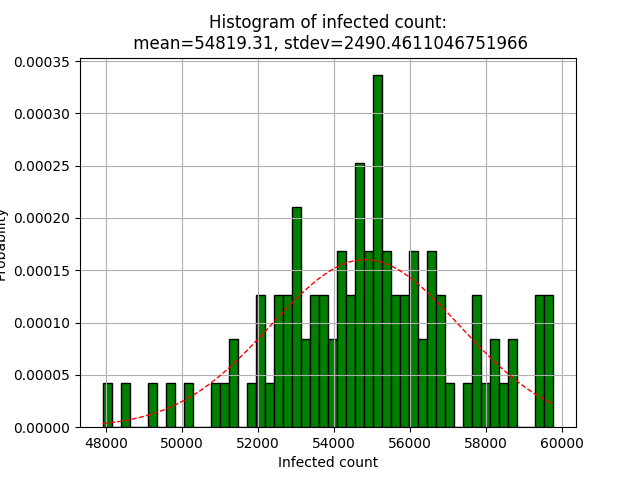
\includegraphics[width=1\linewidth]
  {Measles_12/Measles_12-histogram.png}
  \caption{Histogram of the Meaz1les 12}
  \label{fig:Histogram_Meazles_12}
\end{subfigure}

\begin{subfigure}{.5\textwidth}
  \centering
  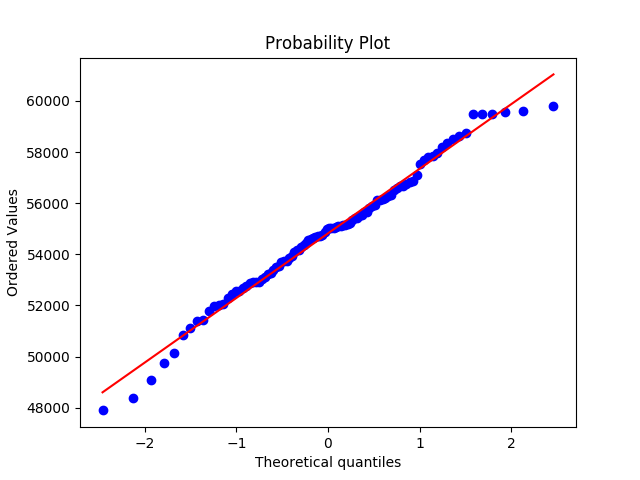
\includegraphics[width=1\linewidth]
  {Measles_12/Measles_12-qqplot.png}
  \caption{QQ-plot of Meazles1 12}
  \label{fig:QQ-plot_Meazles_12}
\end{subfigure}%
\begin{subfigure}{.5\textwidth}
  \centering
  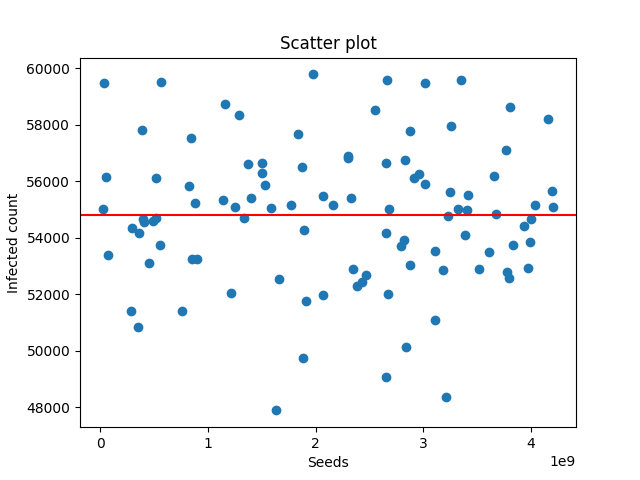
\includegraphics[width=1\linewidth]
  {Measles_12/Measles_12-scatterplot.png}
  \caption{Scatter plot of Measles 12}
  \label{fig:scatterplot_Meazles_12}
\end{subfigure}
\caption{Figures of Measles 12}
\label{fig:Meazles 12}
\end{figure}
\pagebreak
%-----------------------
\subsection{Measles 16}
Stride config file found \href{https://github.com/RobbeHeirman/Config1s/blob/master/config/run_random-geopop_nolog-measles.xml}{here}.\\
Use of this \href{https://github.com/RobbeHeirman/Configs/blob/master/100-random.txt}{seed file}.
\\
\verbatiminput{Measles_16/Measles_16-data.txt}
\begin{figure}[H]
\centering
\begin{subfigure}{.5\textwidth}
  \centering
  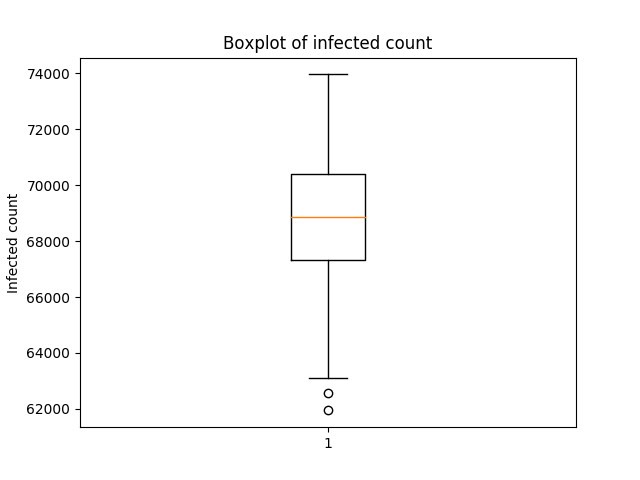
\includegraphics[width=1\linewidth]{Measles_16/Measles_16-boxplot.png}
  \caption{Boxplot Measles 16 runs }
  \label{fig:Boxplot_Measles_16}
\end{subfigure}%
\begin{subfigure}{.5\textwidth}
  \centering
  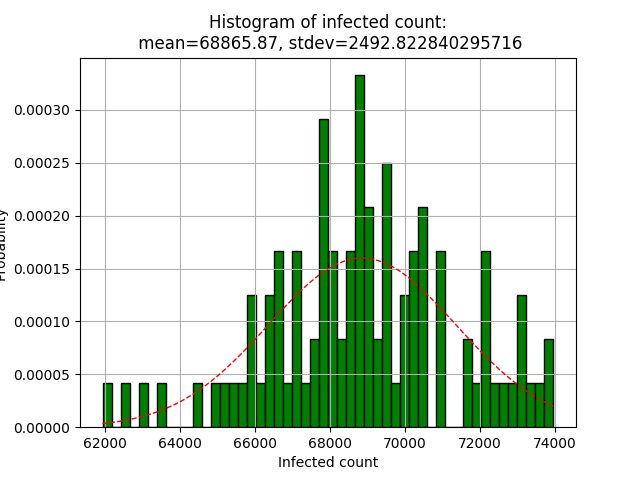
\includegraphics[width=1\linewidth]
  {Measles_16/Measles_16-histogram.png}
  \caption{Histogram of the Meaz1les 16}
  \label{fig:Histogram_Meazles_16}
\end{subfigure}

\begin{subfigure}{.5\textwidth}
  \centering
  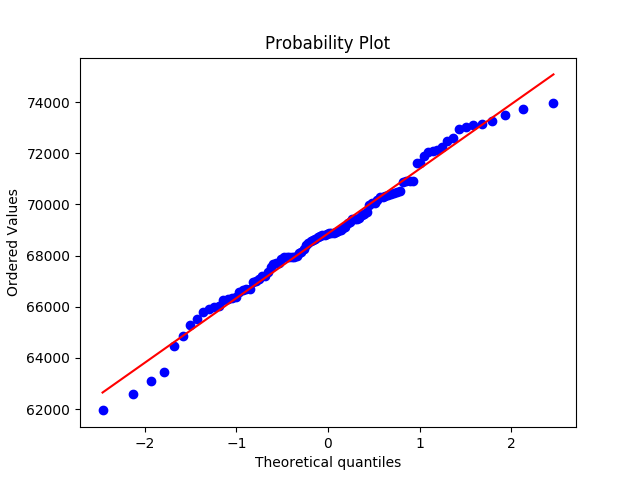
\includegraphics[width=1\linewidth]
  {Measles_16/Measles_16-qqplot.png}
  \caption{QQ-plot of Meazles1 16}
  \label{fig:QQ-plot_Meazles_16}
\end{subfigure}%
\begin{subfigure}{.5\textwidth}
  \centering
  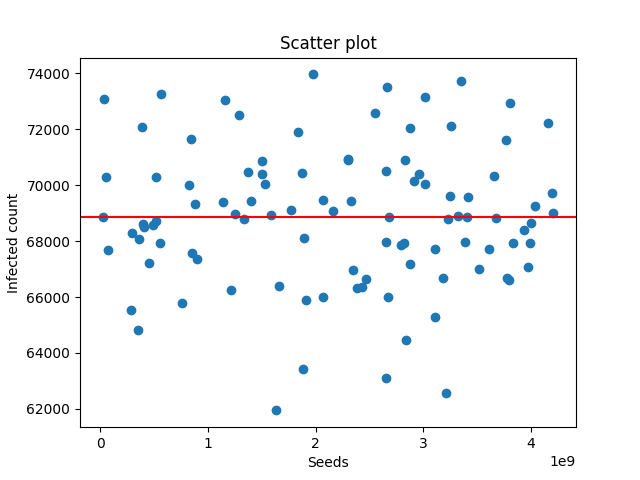
\includegraphics[width=1\linewidth]
  {Measles_16/Measles_16-scatterplot.png}
  \caption{Scatter plot of Measles 16}
  \label{fig:scatterplot_Meazles_16}
\end{subfigure}
\caption{Figures of Measles 16}
\label{fig:Meazles 16}
\end{figure}
\pagebreak
%----------------------------------------------------
\section*{Conclusion}
Something goes wrong when we try to run the Influenza C use case. (Or only five people are susceptible to this disease but this is rather unlikely). The margins we found that we can use in the scenario tests are
\begin{itemize}
\item Influenza A : 0.080
\item Measles 12  : 0.126
\item Measles 16  : 0.100  
\end{itemize}      
Further we can conclude the stochastic spread is according to a normal distribution for the three representative use cases.We do this by checking the QQ plots.
\end{document}